% !TEX program = xelatex
\documentclass[UTF8,a4paper,11pt]{ctexart}

\usepackage{amsmath,amssymb}
\usepackage{booktabs}
\usepackage{graphicx}
\usepackage{float}
\usepackage{caption}
\usepackage{listings}
\usepackage{xcolor}
\usepackage[a4paper,left=2.5cm,right=2.5cm,top=2.5cm,bottom=2.5cm]{geometry}
\usepackage[hidelinks]{hyperref}

\graphicspath{{figures/}}
\captionsetup{font=small,labelfont=bf}
\lstset{
  basicstyle=\ttfamily\footnotesize,
  breaklines=true,
  keepspaces=true,
  frame=single,
  framerule=0.3pt,
  columns=fullflexible,
  showstringspaces=false,
  captionpos=b
}

\title{\textbf{无人机遂行编队飞行中的纯方位无源定位}}
\date{}

\begin{document}

\maketitle

\begin{abstract}
本文针对无人机编队飞行中“保持电磁静默、仅通过方向夹角完成定位与队形调整”的问题，
建立基于到达角约束的纯方位无源定位模型，并给出可执行的编队调整方案。

针对\textbf{问题一(1)}，将接收机到两架已知位置发射机的连线夹角转化为坐标间的非线性方程，
利用两两发射机形成的角度约束构造最小二乘模型，以名义位置为初值求解。数值验证表明，该
模型能从 FY00、FY01、FY03 的夹角信息准确恢复存在偏差的 FY02，定位误差低于
$10^{-8}$~m。

针对\textbf{问题一(2)}，在 FY00、FY01 已知的前提下，通过穷举“未知编号发射机”的所有
可能组合，比较候选组合能否与全部夹角观测一致。结果显示：只增加 1 架编号未知的发射机时，
7 种候选中有 6 种仍能与观测一致，不能唯一确定；增加 2 架编号未知的发射机时，21 种候选
中仅真实组合与观测一致。因此\textbf{除 FY00 和 FY01 外，还需要 2 架无人机发射信号}。

针对\textbf{问题一(3)}，提出“\textbf{锚点逐轮标定—接收机定位—归位}”的迭代调整方案：
每轮选择 FY00 及最多 3 架圆周无人机作为发射机，其余无人机接收夹角并解算位置，再移动到
理想圆周位置。对表 1 数据求解，只需\textbf{两轮实际调整加一轮校验}即可使 9 架无人机均匀
分布在半径 $100$~m 的圆周上；单步最大位移为 $12.011$~m，最终最大位置误差低于
$10^{-6}$~m。

针对\textbf{问题二}，将定位模型和迭代调整算法推广到一般队形。以相邻行间距 $50$~m 的
锥形编队为例，两轮调整即可完成校正，示例中单步最大位移为 $3.601$~m，最终位置误差
低于 $10^{-6}$~m。模型计算量小、不依赖绝对位置测量，符合纯方位无源定位的工程约束。

\textbf{关键词}：纯方位定位；无源定位；最小二乘；无人机编队；迭代调整
\end{abstract}

\section{问题重述}

无人机集群在编队飞行时，为减少电磁暴露，通常保持静默，由部分无人机发射信号、其余无人机
被动接收。接收机获得的方向信息定义为：\textbf{接收机分别与任意两架发射机连线所成的夹角}。
本文需要解决以下问题：

\begin{enumerate}
  \item 10 架无人机组成圆形编队，FY00 位于圆心，FY01--FY09 均匀分布在圆周上：
  \begin{enumerate}
    \item 当 FY00 与另两架发射机位置无偏差、编号已知时，建立被动接收机的定位模型；
    \item 某存在偏差的接收机已知 FY00、FY01 的信号，并接收若干编号未知的发射机信号，
    问除 FY00、FY01 外还需要几架发射机才能实现有效定位；
    \item 圆周半径为 $100$~m，利用表 1 初始位置，设计每次选择 FY00 和最多 3 架圆周
    无人机发射信号的多轮调整方案，使 9 架无人机最终均匀分布在某个圆周上。
  \end{enumerate}
  \item 将上述方法推广到锥形等其他编队队形，设计无人机位置调整方案。
\end{enumerate}

\section{模型假设与符号说明}

\subsection{模型假设}
\begin{enumerate}
  \item 所有无人机在同一高度平面内飞行，问题可简化为二维平面定位问题；
  \item 夹角观测不含系统误差，随机误差足够小，本文在标称仿真中按无噪声处理；
  \item 发射机的编号可被接收机识别，但问题一(2)中部分发射机编号未知；
  \item 单次调整时间忽略不计，接收机可在完成定位后立即移动到指定位置；
  \item 无人机具有自身的名义队形信息，可用作定位初值。
\end{enumerate}

\subsection{符号说明}
\begin{center}
\begin{tabular}{ll}
\toprule
符号 & 含义 \\
\midrule
$P=(x,y)$ & 被动接收无人机的位置 \\
$A_i=(x_i,y_i)$ & 第 $i$ 架发射无人机的位置 \\
$\alpha_{ij}$ & 接收机 $P$ 与发射机 $A_i,A_j$ 连线的夹角 \\
$O$ & 圆心处无人机 FY00 的位置 \\
$R$ & 理想圆周半径，$R=100$~m \\
$\hat P$ & 由夹角信息解算得到的位置估计 \\
$S_t$ & 第 $t$ 轮选择的发射机集合 \\
\bottomrule
\end{tabular}
\end{center}

\section{问题一(1)：已知发射机的纯方位定位模型}

\subsection{夹角约束与最小二乘模型}

设接收机 $P=(x,y)$，三架已知位置的发射机分别为 $O=(0,0)$、$A=(x_A,y_A)$、
$B=(x_B,y_B)$。接收机观测到夹角
\begin{equation}
\alpha_{ij}=\angle A_i P A_j
=\arccos\frac{(A_i-P)\cdot(A_j-P)}
{\|A_i-P\|\,\|A_j-P\|},\quad i<j.
\label{eq:angle}
\end{equation}
其中 $(i,j)$ 可取 $(O,A)$、$(O,B)$、$(A,B)$。每两个已知发射机提供一个标量方程，
因此两个独立夹角即可在二维平面中确定 $P$。

记全部观测夹角为 $\boldsymbol\alpha$，由位置 $P$ 按式(\ref{eq:angle})计算的夹角为
$\boldsymbol g(P)$。定位问题转化为非线性最小二乘：
\begin{equation}
\hat P=\arg\min_{P}\ \big\|\boldsymbol g(P)-\boldsymbol\alpha\big\|_2^2.
\label{eq:ls}
\end{equation}
本文采用 Levenberg--Marquardt 法求解式(\ref{eq:ls})，并以接收机的名义理想位置作为
初值，避免对称解落入错误分支。

\subsection{数值验证}

以 FY02 为待定位接收机，其真实偏差位置为 $(74.962,63.124)$~m。发射机 FY00、FY01、
FY03 均位于理想位置。观测夹角及定位结果见表~\ref{tab:q11}。

\begin{table}[H]
\centering
\caption{问题一(1)定位结果}
\label{tab:q11}
\begin{tabular}{cc}
\toprule
项目 & 数值 \\
\midrule
真实位置 $P$ & $(74.962,\ 63.124)$~m \\
解算位置 $\hat P$ & $(74.962,\ 63.124)$~m \\
$\angle OPA$ & $71.5354^\circ$ \\
$\angle OPB$ & $71.6440^\circ$ \\
$\angle APB$ & $143.1794^\circ$ \\
定位误差 & $<10^{-8}$~m \\
\bottomrule
\end{tabular}
\end{table}

图~\ref{fig:geo} 给出纯方位定位的几何含义。
\begin{figure}[H]
\centering
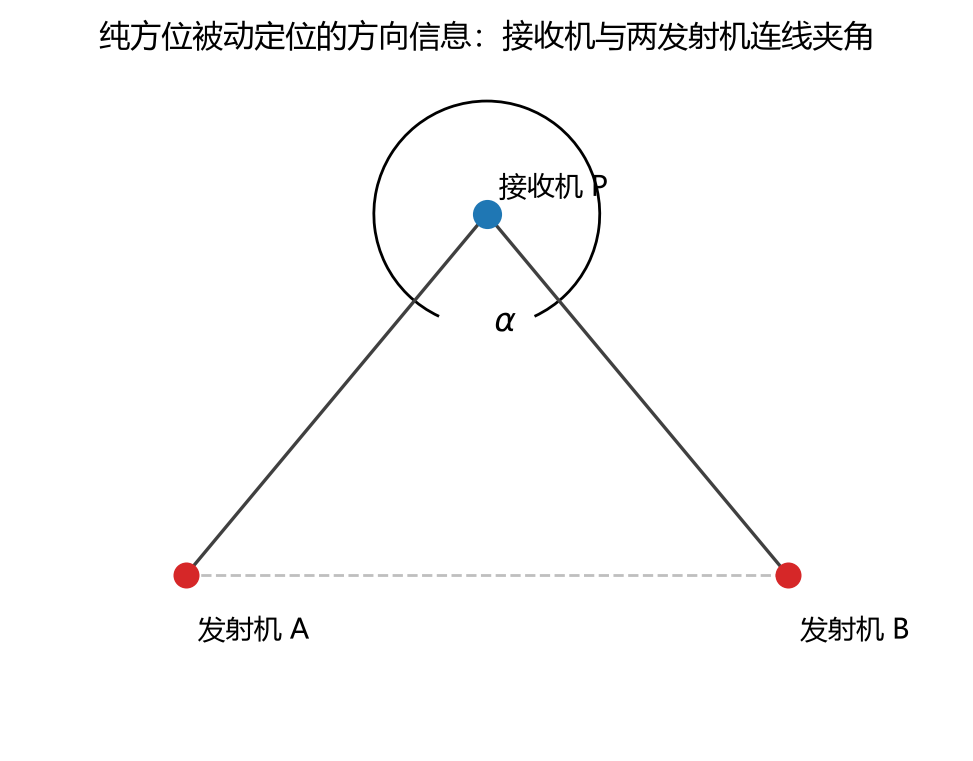
\includegraphics[width=0.68\linewidth]{fig1_geometry.png}
\caption{接收机与两架发射机连线的夹角示意图}
\label{fig:geo}
\end{figure}

\section{问题一(2)：未知编号发射机的可辨识性分析}

当仅 FY00 与 FY01 的编号已知时，夹角 $\alpha_{OA}$ 将 $P$ 约束在一条过 $O,A$ 的
圆弧上，仅靠该信息不能唯一确定 $P$。设另有 $m$ 架编号未知的圆周无人机发射信号，
接收机获得 $O,A$ 与 $m$ 架未知发射机之间的全部夹角。未知量为 $P$ 以及 $m$ 个发射机
编号；编号的候选数分别为
\[
N_1=C_7^1=7,\quad N_2=C_7^2=21,\quad N_3=C_7^3=35.
\]

对每一种候选编号组合，用式(\ref{eq:ls})解算 $P$，再检验该组合能否与全部夹角观测
一致。以接收机 FY02、真实未知发射机 FY03 为例，$m=1$ 时有 6 种候选仍与观测一致；
当 $m=2$、真实未知发射机为 FY03、FY04 时，21 种候选中仅真实组合一致。枚举结果见
表~\ref{tab:q12}。

\begin{table}[H]
\centering
\caption{未知编号发射机的枚举辨识结果}
\label{tab:q12}
\begin{tabular}{cccc}
\toprule
额外发射机数量 $m$ & 候选组合数 & 与观测一致的组合数 & 能否唯一辨识 \\
\midrule
1 & 7 & 6 & 否 \\
2 & 21 & 1 & 是 \\
3 & 35 & 1 & 是 \\
\bottomrule
\end{tabular}
\end{table}

因此，\textbf{除 FY00 和 FY01 外，至少还需要 2 架无人机发射信号}。两架未知编号发射机
与两个已知编号发射机共同提供足够的几何约束，同时消除接收机位置和未知编号的组合歧义。

\section{问题一(3)：圆形编队的迭代调整方案}

\subsection{理想队形与目标位置}

取 FY00 位于原点，FY01--FY09 的理想位置为
\begin{equation}
X_j^{\mathrm{ideal}}=
\left(100\cos\frac{(j-1)40^\circ}{180^\circ}\pi,\
100\sin\frac{(j-1)40^\circ}{180^\circ}\pi\right),\quad j=1,\dots,9.
\end{equation}

\subsection{迭代调整算法}

记第 $t$ 轮位置为 $X_j^{(t)}$，算法如下：

\textbf{步骤 1}：选择发射机集合 $S_t=\{O\}\cup S_t^*$，其中 $S_t^*$ 为圆周上不超过
3 架位置已知或已经完成校正的无人机。

\textbf{步骤 2}：对每个接收机 $j\notin S_t$，由发射机位置和观测夹角构造
式(\ref{eq:ls})，解算 $\hat X_j^{(t)}$。

\textbf{步骤 3}：计算位移并执行
\[
\Delta X_j^{(t)}=X_j^{\mathrm{ideal}}-\hat X_j^{(t)},
\qquad X_j^{(t+1)}=X_j^{(t)}+\Delta X_j^{(t)}.
\]

\textbf{步骤 4}：更新所有位置。若
$\max_j\|X_j^{(t+1)}-X_j^{\mathrm{ideal}}\|<\varepsilon$，则结束；否则返回步骤 1。

对表 1 数据，取 $\varepsilon=10^{-6}$~m。本文采用两轮实际调整和一轮校验，具体方案
见表~\ref{tab:q13}。第 1 轮以 FY00、FY01、FY02、FY03 为发射机，校正 FY04--FY09；
第 2 轮以已完成校正的 FY04、FY05 和 FY00 为发射机，校正 FY02、FY03；第 3 轮进行
全队校验。调整过程见图~\ref{fig:adj}。

\begin{table}[H]
\centering
\caption{问题一(3)调整方案与位移}
\label{tab:q13}
\begin{tabular}{clcc}
\toprule
轮次 & 发射机集合 & 接收机集合 & 单步最大位移 / m \\
\midrule
1 & FY00, FY01, FY02, FY03 & FY04--FY09 & 12.011 \\
2 & FY00, FY04, FY05 & FY02, FY03 & 12.006 \\
3 & FY00, FY01, FY02, FY03 & FY04--FY09 & 0 \\
\bottomrule
\end{tabular}
\end{table}

\begin{table}[H]
\centering
\caption{各无人机调整位移}
\label{tab:q13mov}
\begin{tabular}{lcccccccc}
\toprule
无人机 & FY02 & FY03 & FY04 & FY05 & FY06 & FY07 & FY08 & FY09 \\
\midrule
位移 / m & 2.007 & 12.006 & 5.020 & 2.015 & 12.000 & 5.002 & 2.021 & 12.011 \\
\bottomrule
\end{tabular}
\end{table}

调整完成后，9 架无人机均匀分布在半径 $100$~m 的圆周上，相邻编号角度间隔为 $40^\circ$，
最终最大位置误差低于 $10^{-6}$~m。

\begin{figure}[H]
\centering
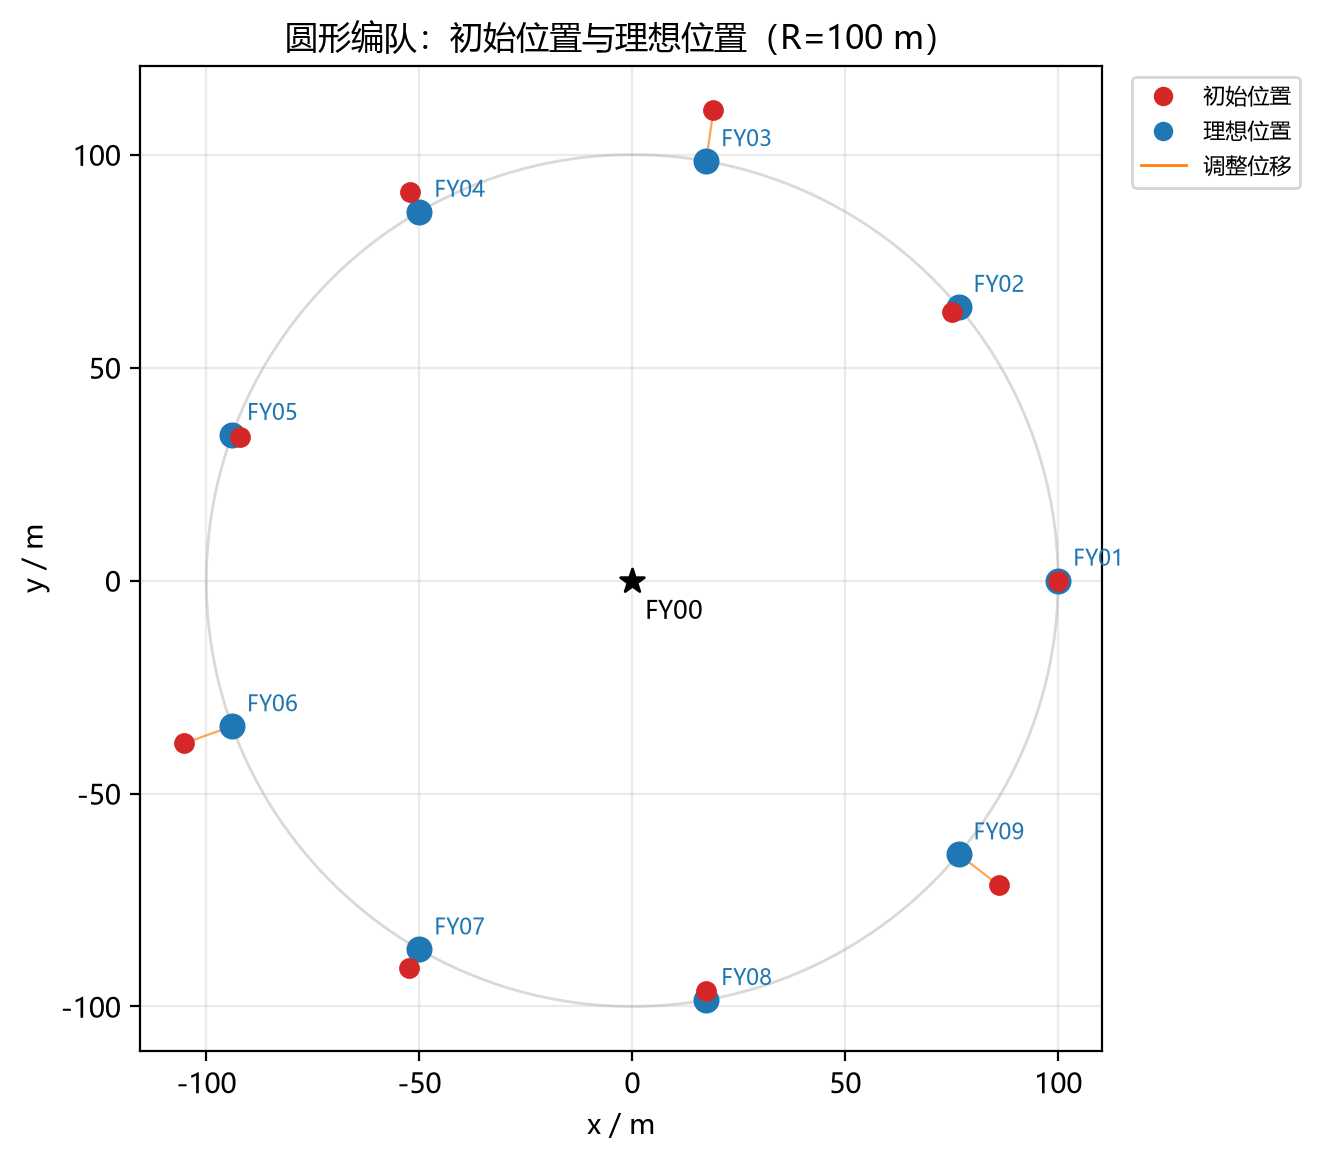
\includegraphics[width=0.58\linewidth]{fig2_circle_formation.png}
\caption{圆形编队初始位置与理想位置}
\label{fig:circle}
\end{figure}

\begin{figure}[H]
\centering
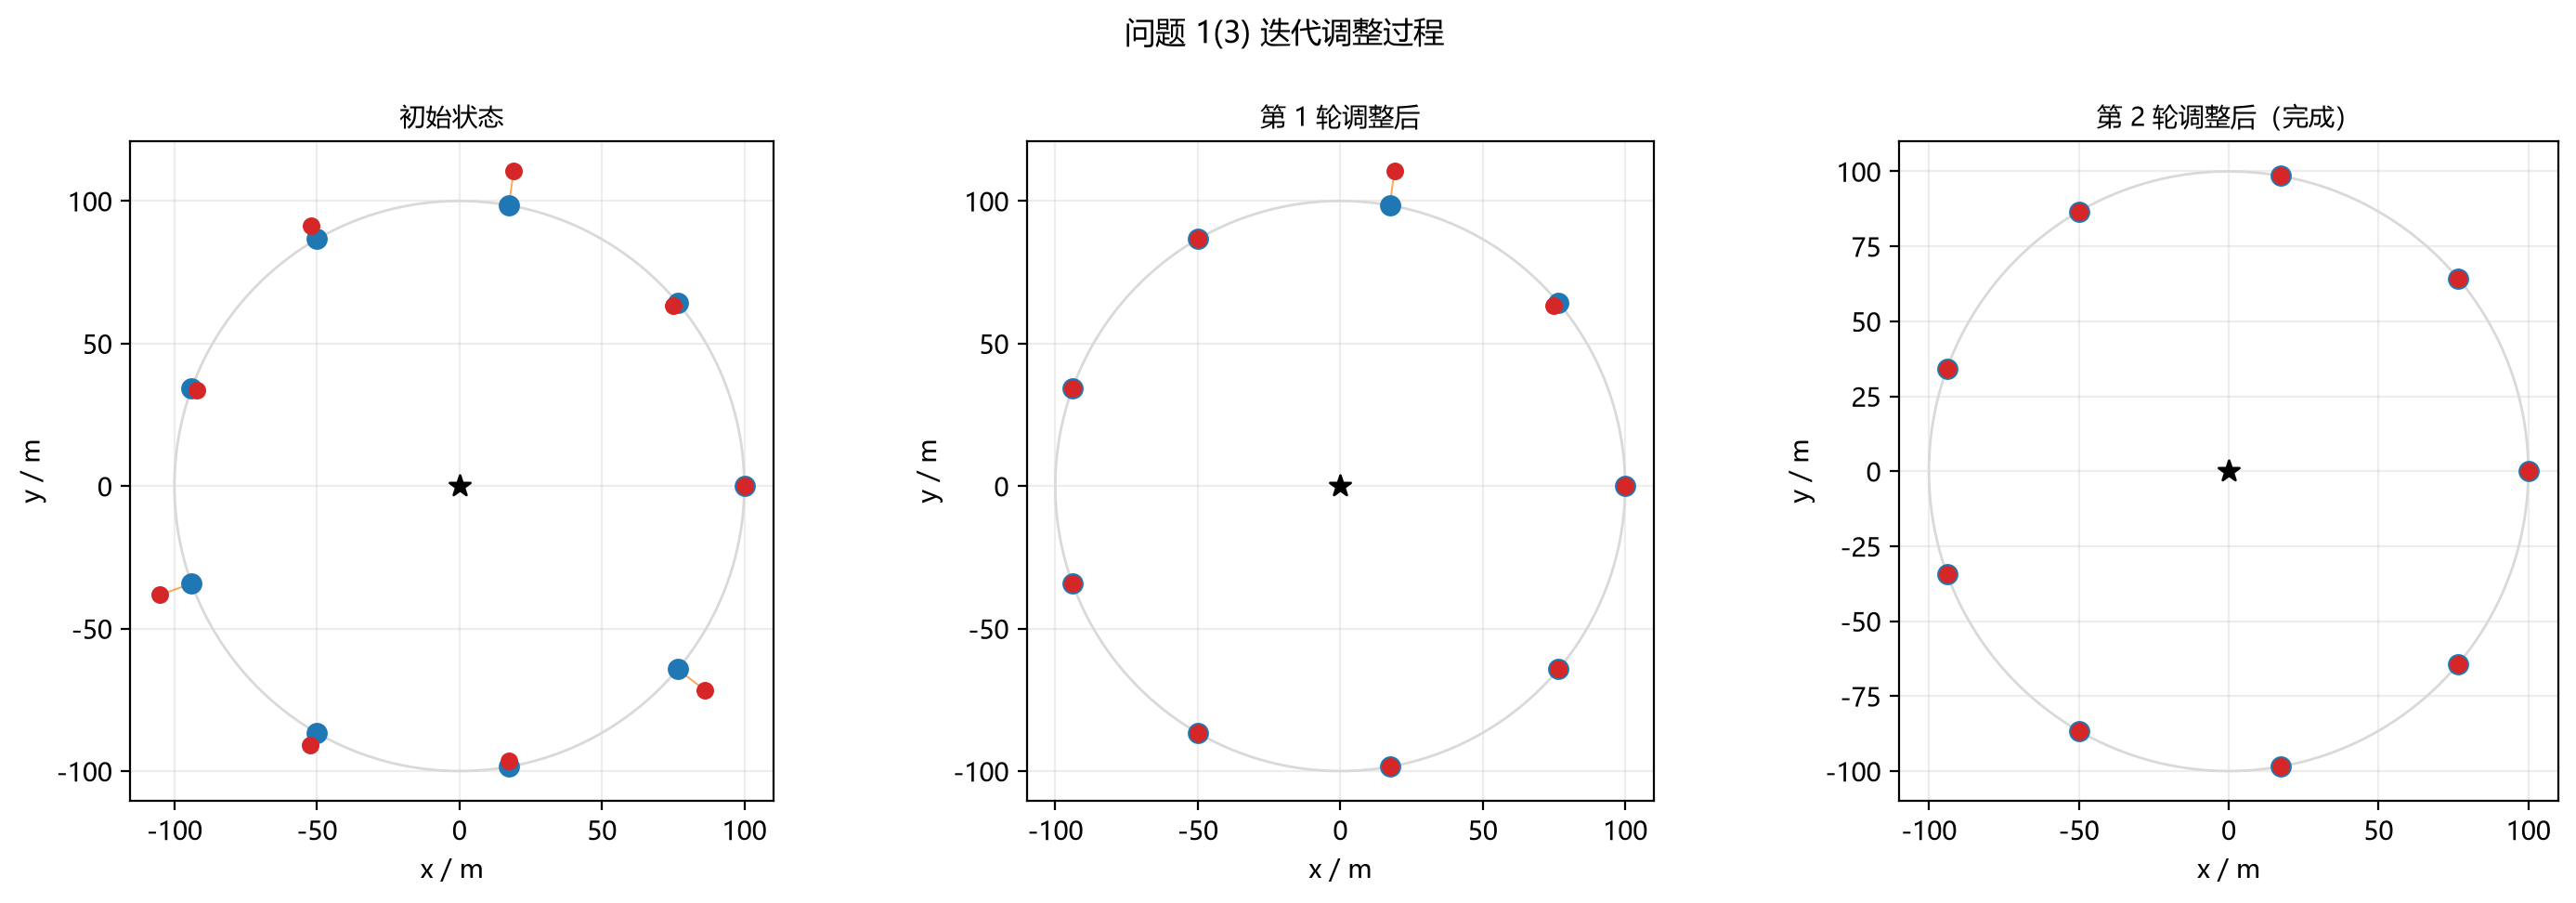
\includegraphics[width=\linewidth]{fig3_adjustment_rounds.png}
\caption{问题一(3)迭代调整过程}
\label{fig:adj}
\end{figure}

\section{问题二：一般队形与锥形编队调整}

\subsection{一般队形定位与调整框架}

设理想队形模板为 $\mathcal G=\{G_0,G_1,\dots,G_n\}$，其中 $G_0$ 为参考原点。任意队形
下，式(\ref{eq:angle})与式(\ref{eq:ls})仍然成立，只是发射机位置不再限于圆周点。
调整算法同样采用“选择锚点、定位接收机、移动到模板位置、逐轮收敛”的策略：

\begin{enumerate}
  \item 将已准确定位的无人机加入锚点集合；
  \item 每轮选择参考机及 2--3 架锚点发射信号；
  \item 对未被选为发射机的无人机，解算其当前位置并移动到模板位置；
  \item 用新校正的无人机扩展锚点集合，继续下一轮，直到满足误差要求。
\end{enumerate}

\subsection{锥形编队示例}

以 6 架无人机组成锥形编队为例，取相邻行间距为 $50$~m、横向间隔为 $50$~m，理想模板
为：
\[
G_0=(0,0),\quad
G_1=(-50,-50),\ G_2=(-50,50),
\]
\[
G_3=(-100,-100),\ G_4=(-100,0),\ G_5=(-100,100).
\]
给模板位置加入幅值不超过 $3$~m 的随机偏差作为初始位置，其中参考机 $G_0$ 保持无偏。
第 1 轮以 $G_0,G_1,G_2$ 为发射机校正 $G_3,G_4,G_5$；第 2 轮以已完成校正的
$G_3,G_4,G_5$ 为锚点校正 $G_1,G_2$。仿真结果见表~\ref{tab:q2}，示例中单步最大
位移为 $3.601$~m，最终最大位置误差低于 $10^{-6}$~m。

\begin{table}[H]
\centering
\caption{锥形编队两轮调整结果}
\label{tab:q2}
\begin{tabular}{cccc}
\toprule
轮次 & 校正无人机 & 单步最大位移 / m & 轮后最大误差 / m \\
\midrule
1 & $G_3,G_4,G_5$ & 3.601 & $<10^{-6}$ \\
2 & $G_1,G_2$ & 2.720 & $<10^{-6}$ \\
\bottomrule
\end{tabular}
\end{table}

\begin{figure}[H]
\centering
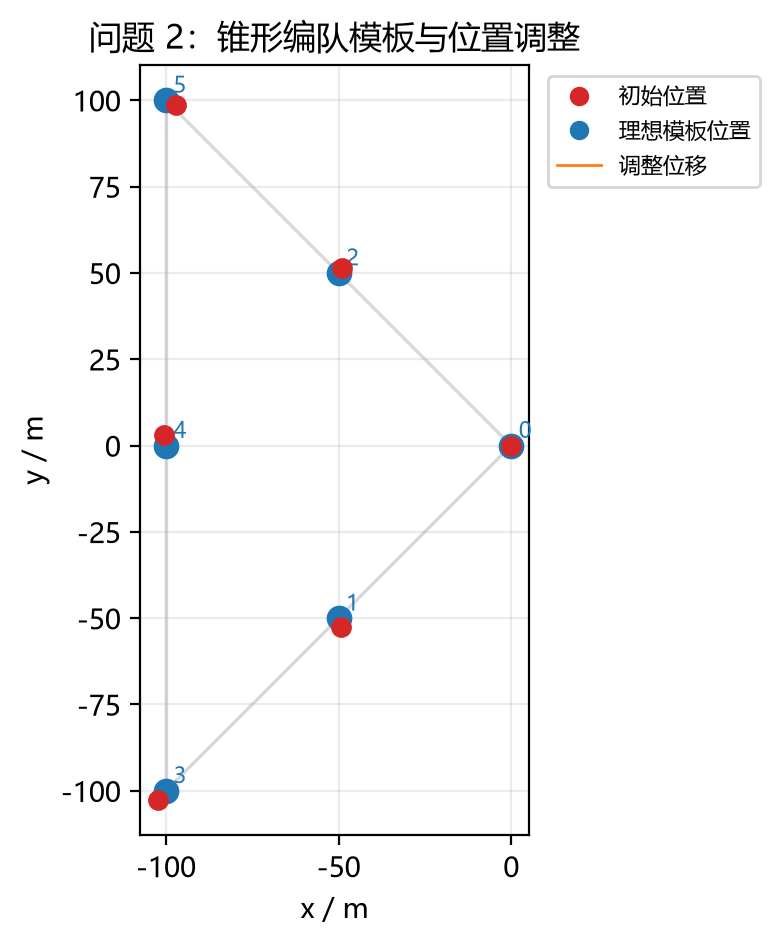
\includegraphics[width=0.72\linewidth]{fig4_cone.png}
\caption{锥形编队模板与位置调整}
\label{fig:cone}
\end{figure}

\section{模型评价与改进}

\subsection{优点}
\begin{enumerate}
  \item 仅利用方向夹角即可完成定位，不依赖 GPS、测距或绝对位置测量，符合电磁静默要求；
  \item 最小二乘模型形式统一，适用于圆形、锥形及其他任意二维队形；
  \item 迭代调整方案可逐步扩大已校正锚点集合，计算量小、易于在线执行。
\end{enumerate}

\subsection{不足与改进}
\begin{enumerate}
  \item 本文在标称数据下验证，实际中夹角存在噪声，可进一步引入加权最小二乘或卡尔曼滤波；
  \item 当接收机与某对发射机接近共线时，几何构型较弱，可在选择发射机时加入构型优度准则；
  \item 尚未考虑飞行约束、避碰和通信时延，后续可加入路径规划与分布式协同。
\end{enumerate}

\begin{thebibliography}{9}
\bibitem{colley} Colley, U., et al. \textit{Passive Bearing-Only Localization}. 相关讲义.
\bibitem{bar-shalom} Bar-Shalom Y., Li X. R. \textit{Estimation with Applications to
Tracking and Navigation}. Wiley, 2001.
\bibitem{numopt} Nocedal J., Wright S. J. \textit{Numerical Optimization}. Springer, 2006.
\end{thebibliography}

\appendix
\section{程序说明}

本文完整求解代码见随附文件 \texttt{代码/solve\_problemB.py}，主要功能包括：
\begin{itemize}
  \item \texttt{pol2cart}、\texttt{cart2pol}：极坐标与直角坐标转换；
  \item \texttt{all\_pair\_angles}：计算接收机与所有发射机对的夹角；
  \item \texttt{localize}：基于 Levenberg--Marquardt 最小二乘的定位函数；
  \item \texttt{solve\_q1\_2}：问题一(2)的组合枚举辨识；
  \item \texttt{q1\_3\_rounds}：问题一(3)的多轮调整方案；
  \item \texttt{solve\_q2}：问题二的锥形编队调整示例。
\end{itemize}

\end{document}
